\section{Bottom-up block failure modeling}
\label{sec:bottom-up-modeling}

\subsection{Block failure characterization and modeling method}
\label{sec:block-failure-cz}

% What is bottom up
The modeling method presented in this section focuses first on studying low-level cells of the circuit.
They are characterized individually, leading to the definition of a failure model for each cell.
In a second step, the individual models are linked together.
The connection between the models reproduce the connections between the cells in the actual circuit.
Finally, an electrical stimulus such as an electrostatic discharge is fed on the input of the first model.
It is applied on this model that produces an output signal.
In turn, this signal is used as stimulus for the second model in the chain which is using it as input.
The process is repeated until the last output, where the output signal represents the shape of the disturbance after going through the entire chain.

% Why bottom up
The main perk of this characterization method is the modularity, because each block is characterized independently of the others.
The model built for each cell is reusable, and once the characterization is done it does not need to be repeated unless modifications are brought to the circuit.
This method is called bottom-up because low-level functions components are characterized then assembled to model higher-level functions, rising from the bottom of the hierarchy to upper levels.

% Why modelling individual blocks
The motivation for modeling blocks individually is that a single block can be failing but the error can remain internal.
Complete function can continue to operate without changes.
In the other way around, not all blocks need to be failing in order to cause the complete function to fail as well.
It is important to determine which blocks may be in fault to be able to fix the problem.
This is why the characterization method presented here focuses on blocks and not complete functions.

% Models are not electrical but failure models
The goal of this method is to build a propagation model and not an electrical \gls{spice} model.
The models built here are not usable directly in standard simulations and does not produce strict waveforms on their outputs.
Instead, they represent input and output waveforms by bounding boxes of a given amplitude and width.
The methodology is built on the hypothesis that simplified \gls{esd} waveforms could be sufficient to estimate the robustness of an integrated function.
This hypothesis is tested as detailed later in the document.

% Describe the changes
Several refinements of the modeling methods were applied to solve issues as they were encountered.
This chapter gives a logical history of those improvements in order to understand the starting phase and the modifications applied after.
Initially, Wunsch and Bell characterization \cite{wunsch-bell} is used to determine failure levels of individual cells when exposed to stresses of different width and amplitude.
A single failure criteria was preliminary established for each model.
It usually took the form of a voltage threshold applied on the output of a cell, above which a fault is recorded.
This threshold is set prior to the simulation, and there is no general rule for setting it.
The \gls{dc} specification of the output can be used directly, if it exists, or a sound value in regard of the design, or an arbitrary level.

% How is it done, core concept
The first part of the modeling method is the characterization of each block using the electrical setup of Fig. \ref{block_function_cz} in a \gls{spice} simulation environment.
This setup provides appropriate biasing to the block with V\textsubscript{DC} voltage source, in order to set the block function in operating conditions.
It also enables the injection of the characterization signal on the tested input with V\textsubscript{stress} transient voltage source.
The characterization pulses are rectangular waveforms similarly to the Wunsch and Bell technique.
Each simulation runs with a different pair of values for the \textbf{amplitude} and \textbf{duration} of the square signal.
On the other side of the cell under test, the output is monitored.
Prior to the simulation, a failure criteria consisting of a voltage threshold is set.
If the output waveform goes above this threshold, the simulation is tagged as \textit{fail}.
The threshold is chosen depending on multiple parameters such as the functionality of the block or its DC operating point.

\begin{figure}[!h]
  \centering
  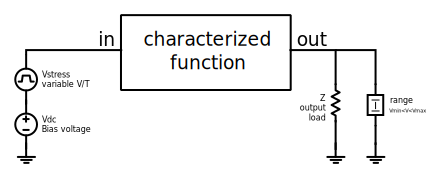
\includegraphics{src/4/figures/characterization_setup.pdf}
  \caption{Block characterization setup (supply input)}
  \label{block_function_cz}
\end{figure}

The results are summarized into table \ref{simulation-results}.
The simulations in red contain a fail, meaning that the output voltage crossed the failure threshold.

\begin{table}[!h]
\centering
\begin{tabular}{@{}lllll@{}}
\toprule
               & \SI{1}{\nano\second}         & \SI{10}{\nano\second}        & \SI{100}{\nano\second}       & \SI{1}{\micro\second}        \\ \midrule
\SI{15}{\volt} & {\color[HTML]{FE0000} sim13} & {\color[HTML]{FE0000} sim23} & {\color[HTML]{FE0000} sim33} & {\color[HTML]{FE0000} sim43} \\
\SI{10}{\volt} & {\color[HTML]{32CB00} sim12} & {\color[HTML]{FE0000} sim22} & {\color[HTML]{FE0000} sim32} & {\color[HTML]{FE0000} sim42} \\
\SI{5}{\volt}  & {\color[HTML]{32CB00} sim11} & {\color[HTML]{32CB00} sim21} & {\color[HTML]{32CB00} sim31} & {\color[HTML]{FE0000} sim41} \\
\bottomrule
\end{tabular}
\caption{Example of results on a set of simulations}
\label{simulation-results}
\end{table}

% A first visualization of the characterization
A curve can be built from this table to give a visual representation of the functional robustness of the block (see Fig. \ref{wb_cz_curve_example}).
The x axis is the duration of the input stress.
The y axis is the amplitude of the input signal during the stress.
The color of the curve (red or green) corresponds to the presence or absence of failure at the given input amplitude and width.

\begin{figure}[!h]
  \centering
  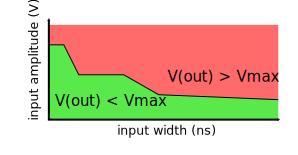
\includegraphics{src/4/figures/example_curve.pdf}
  \caption{Visual representation of powered-on block testing results}
  \label{wb_cz_curve_example}
\end{figure}

% How to improve the displayed information
Presence or absence of a failure is not the only information that can be obtained by monitoring the output.
Because soft-failures are temporary issues, their duration is also very relevant.
Using the same characterization setup as before (Fig. \ref{block_function_cz}), it is possible to also measure the duration of a failure.
It is possible to improve table \ref{simulation-results} by replacing the fail or no-fail flag by the duration of the fail.
This is illustrated in table \ref{simulation-results-bis}.
With those example values, for an input pulse stress of \SI{5}{\volt} with a input pulse width of \SI{1}{\nano\second}, no failure was recorded.
On the other hand, with a \SI{5}{\volt} \SI{1}{\micro\second} stress, a failure was recorded and the output waveform crossed the threshold during \SI{2}{\micro\second}.
A \SI{15}{\volt} \SI{2}{\micro\second} stress caused a failure that lasted \SI{30}{\micro\second}.

\begin{table}[!h]
\centering
\begin{tabular}{@{}lcccc@{}}
\toprule
                & \SI{1}{\nano\second}         & \SI{10}{\nano\second}        & \SI{100}{\nano\second}                        & \SI{1}{\micro\second}     \\ \midrule
\SI{15}{\volt} & {\color[HTML]{00D2CB}110 ns} & {\color[HTML]{FFCB2F}150 ns} & {\color[HTML]{FE0000}\SI{30}{\micro\second}}  & {\color[HTML]{FE0000} \SI{30}{\micro\second}} \\
\SI{10}{\volt} & {\color[HTML]{32CB00}}       & {\color[HTML]{00D2CB}125 ns} & {\color[HTML]{F8A102}540 ns}                  & {\color[HTML]{FE0000} \SI{30}{\micro\second}} \\
\SI{5}{\volt}  & {\color[HTML]{32CB00}}       & {\color[HTML]{32CB00} }      & {\color[HTML]{32CB00} }                       & {\color[HTML]{F56B00} \SI{2}{\micro\second}}  \\
\bottomrule
\end{tabular}
\caption{Example result set containing failure width information}
\label{simulation-results-bis}
\end{table}

% How to improve the curve from the improved table
This improvement can also be transfered to the curve representation.
A gradient is used rather than a fail or no-fail area.
The gradient color for each location corresponds to the failure duration the output.
The figure \ref{wb_cz_curve_example_v2} provides an example of this improved representation.
In this figure, the warmer the gradient, the longer the output is disturbed.

\begin{figure}[!h]
  \centering
  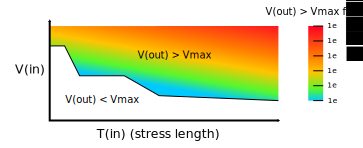
\includegraphics{src/4/figures/example_curve_v2.pdf}
  \caption{Improved curve for Wunsch and Bell powered-on characterization}
  \label{wb_cz_curve_example_v2}
\end{figure}

The gradient can also be discretized into a few areas for better readability as shown in figure \ref{wb_cz_curve_example_v2_discrete}.
This representation looses some information compared to the gradient one but is easier to generate and read.

\begin{figure}[!h]
  \centering
  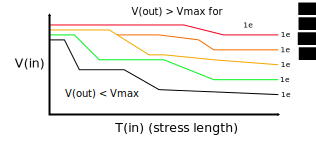
\includegraphics{src/4/figures/example_curve_v2_discrete.pdf}
  \caption{Improved discrete curve for Wunsch and Bell powered-on characterization}
  \label{wb_cz_curve_example_v2_discrete}
\end{figure}

% Summarize the method
In this section, a method was detailed to extract the robustness of a block function.
It relies on injecting pulses on an input and watching for changes on an output.
After characterization, a model can be constructed.
It is composed of a characterization table and a failure criteria.
Fig. \ref{fig:principle-transfert-func} provides a visual representation of this model.

\begin{figure}[!h]
  \centering
  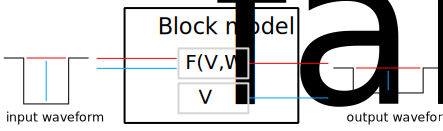
\includegraphics[width=0.8\textwidth]{src/4/figures/principle_transfert_function.pdf}
  \caption{First modeling method}
  \label{fig:principle-transfert-func}
\end{figure}

% Explain the visual representation
The model accepts a rectangular input waveform and returns a rectangular output waveform (Fig. \ref{fig:principle-transfert-func}).
More specifically, the width (red arrow) and the amplitude (blue arrow) of the input signal are the two parameters required by the model.
Those values are fed to the characterization table to calculate the width of the output signal.
The characterization table is represented by the function $F(V,W)$, with $V$ corresponding to the input amplitude and $W$ to the input width.
The failure criteria V\textsubscript{fail}, employed for establishing the characterization table, is also used directly as amplitude value for the output signal.
Using the failure criteria for modeling the output amplitude is a large approximation and validity of this approach is checked in the next section.
Ultimately, the goal is to investigate whether or not a fixed failure threshold is suitable for ESD functional analysis.

% What is done next
In the next section, those individual block models are chained together to deduce the robustness of a complete function.
The processed is explained in detailed and is later applied on a practical case.

\subsection{Block models chaining}
\label{sec:block-chaining}

% Explain the chaining mechanism
This section presents the second phase of the method that consists in chaining individual block models to deduce the robustness of a higher-level function.
To present this concept of chaining models, a purely hypothetical example is taken first.
The method is tested with a true case study afterwards.
The characterization process detailed previously is performed on two different blocks, called $A$ and $B$ (see Fig. \ref{example_toplevel_function}).
Those two blocks are part of an hypothetical higher-level function.
The function has an external input (called \textit{in}) and an external output (called \textit{out}).
A stimulus is injected on the external input and the job of the model chain is to predict what will be the approximate waveform on the external output.
Both blocks were previously (hypothetically) characterized and failure criteria V\textsubscript{fail} for block $A$ is \SI{5}{\volt} and \SI{2}{\volt} for block $B$.
In practice, the threshold selection is done either from the block specification or datasheet, or directly from its design.

\begin{figure}[!h]
  \centering
  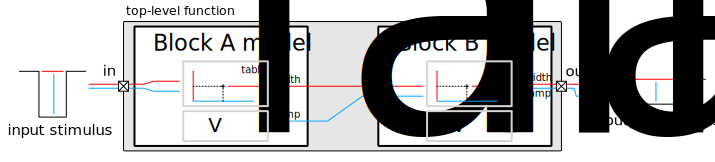
\includegraphics[width=\textwidth]{src/4/figures/example_top_level_function.pdf}
  \caption{Top-level function model constituted of 2 blocks}
  \label{example_toplevel_function}
\end{figure}

% What is the input stress
The input stimulus is a rectangular \SI{100}{\nano\second} wide pulse with a \SI{15}{\volt} amplitude.
Those two properties are fed into the hypothetical characterization of block $A$ (Fig. \ref{example_complete_curve}).
In the graph, multiple curves can be identified, each corresponding to a boundary between two disturbance durations.
For a point located below the green curve (with label "\SI{10}{\nano\second}"), no stress was recorded on the output.
For a point located above the \SI{10}{\nano\second} curve and below the \SI{100}{\nano\second} curve, a stress was indeed recorded with a duration comprised between \SI{10}{\nano\second} and \SI{100}{\nano\second}.
The exact value between those two boundaries is not known with this this kind visualization.
In the analysis, the lower boundary is always chosen because the output is disturbed for at least this value.

\begin{figure}[!h]
  \centering
  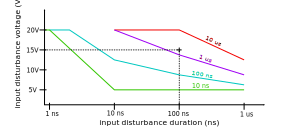
\includegraphics{src/4/figures/example_complete_curve.pdf}
  \caption{Model A curve and determination of impact of the TLP pulse - values in color represent the duration of failure on the output}
  \label{example_complete_curve}
\end{figure}

% Interpretate stress to deduce net1
With the given \SI{15}{\volt} \SI{100}{\nano\second} stimulus, the curve predicts that the output will fall below \SI{5}{\volt} (V\textsubscript{fail} of block A) during \SI{1}{\micro\second}.
Those two values describe the signal on the output of block A.
Those values are now used to describe the stimulus on block B, since both blocks are connected.
The failure criteria that was used to extract the characterization curve also serves as amplitude for the output signal.
It means that with a \SI{5}{\volt} failure criteria, if a failure is recorded, the output waveform is approximated to also have an amplitude of \SI{5}{\volt}.

% Use net1 as input of next block
Fig. \ref{example_complete_curve_B} shows an example curve for model B.
The location of the stimulus from block A (\SI{5}{\volt} and \SI{1}{\micro\second}) is also placed on the curve.
The curve predicts that with this stimulus, block B will be disturbed during \SI{10}{\micro\second} with an amplitude of \SI{2}{\volt} (V\textsubscript{fail} of block B).

\begin{figure}[!h]
  \centering
  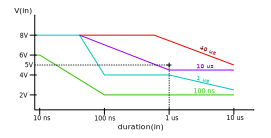
\includegraphics{src/4/figures/example_complete_curve_B.pdf}
  \caption{Model B curve and determination of impact of the TLP pulse}
  \label{example_complete_curve_B}
\end{figure}

% Repeatable process
This process can be repeated in theory with as many blocks as required by the original design, until the final pin is reached.
